\chapter{Using Nonlinear Time Reversal for Selective Reconstructions}
\label{ch:selective}

\section{Purpose}
\label{sec:selective-purpose}

When a WPT system is constructed, it could be advantageous to control which receivers in range are the recipients of electrical power. Linear time reversal is useful for targeting a single device, due to the ability to focus on a single receiver. Tracking several receivers and then independently transmitting them energy poses a significant challenge. Part of this difficulty stems from the fact that the transmitter must have some unique information about the receivers to actually select a desired target. One way to do this is to use receivers which have distinguishing features so the transmitter can select the specific devices. Nonlinear Time Reversal (NLTR) is a version of LTR that creates such distinguishing features in the receivers using nonlinear elements and does not allow unwanted devices to receive more than a negligible amount of energy.

The time-reversal mirror fidelity requires a set of discrete paths between the transmitters and receivers, with neither party knowing the location of the other within the enclosure. The team investigated the case where the receivers differ in their frequency response to an interrogation signal.

\section{Methodology}
\label{sec:selective-meth}

To investigate whether a TR technique can demonstrates the ability to distinguish between receiving targets on a basis of their frequency response to an interrogation signal. These experiments were performed within the Gigabox resonant cavity used in the LTR setup above. The AWG, PSG, and DSO setup are used to receive and transmit signals in a manner similar to their use in the LTR setup. The NLTR setup uses three input/output ports; one representing the sender, and two representing different receivers. The NLTR setup is described in Figure~\ref{fig:selective-setup}.

\begin{figure}[t]
\centering
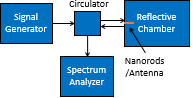
\includegraphics[width=0.85\textwidth]{nonlinear/setup}
    \caption[Selective Targeting Setup]{Selective Targeting Setup}
    \label{fig:selective-setup}
\end{figure}

The two receivers are designated as either ``linear'' or ``nonlinear'' according to their response to a signal at a carrier frequency. The linear receiver responds to the interrogation with a signal at the same carrier frequency as it was queried with. The nonlinear receiver responds with a signal includes the second harmonic of the carrier frequency, in addition to the carrier frequency itself. When an interrogation pulse is transmitted from the sender to both receivers, it is met with a combination of responses at two discrete frequencies; filtering can be used to easily isolate one from the other.

Creating ideal reflector antennas proved to be very difficult given the resources of the team.  Instead of reflectors, an initial signal was broadcast from the receiving antennas.  The nonlinear receiver was routed through a frequency multiplier to create the second harmonic needed for NLTR.  The sona created by the two receivers was collected at the transmitting antenna.  The time reversed sona, broadcast from the transmitting antenna, reconstructs on both of the receivers.  One receiver can be targeted separately by filtering the appropriate frequency from the sona, and broadcasting it alone. A reconstruction should appear at the corresponding receiver's port while the other receiver will only detect noise. To ensure that selective reconstruction occurred, the resulting signals at both receivers were monitored and the presence of a reconstruction (or lack thereof) noted. 

The experiment was performed with Gaussian interrogation pulses 50~ns in length, at a carrier frequency of 4.2~GHz. The sonas were recorded to lengths of 15~$\mu$s and the signals were broadcast at a power of 3~dBm.

\section{Results}
\label{sec:selective-results}

\begin{figure}[h]
\centering
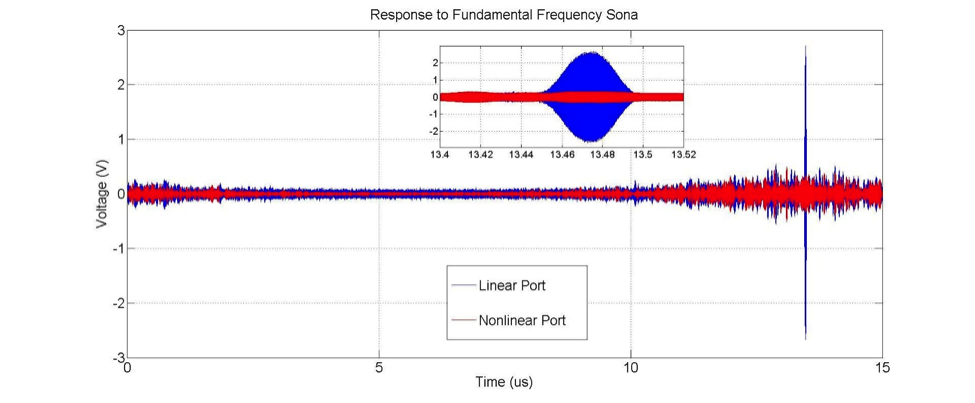
\includegraphics[width=0.85\textwidth]{nonlinear/selective-fundamental}
    \caption[Selective Targeting Linear Port]{Voltage v. Time while Targeting Linear Port}
    \label{fig:selective-fundamental}
\end{figure}
\begin{figure}[h]
\centering
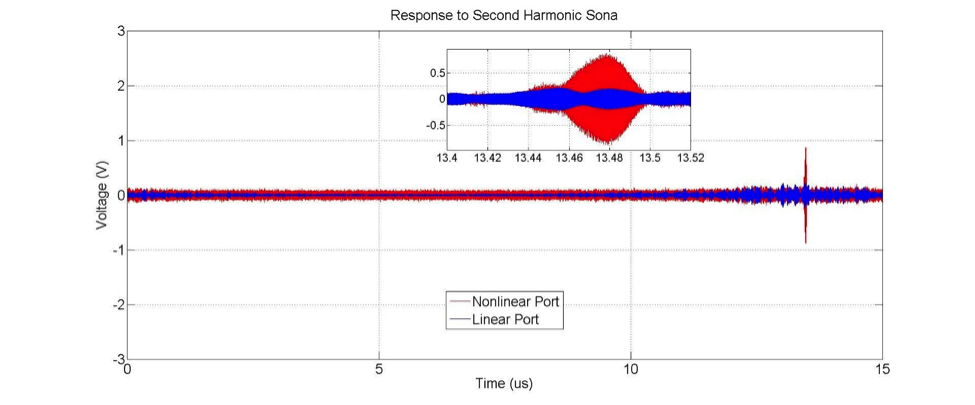
\includegraphics[width=0.85\textwidth]{nonlinear/selective-harmonic}
    \caption[Selective Targeting Nonlinear Port]{Voltage v. Time while Targeting Nonlinear Port}
    \label{fig:selective-harmonic}
\end{figure}

The results of this experiment confirmed the fidelity of the time reversal mirror and its ability to selectively transmit power to a receiver. Monitoring the voltage response of both the linear port and the nonlinear port confirmed the existence of a reconstruction for each case.

When the sona was filtered and broadcast at the linear, carrier frequency, a clear reconstruction emerged at the linear port. At the nonlinear receiver, the lack of a comparable reconstruction is notable. The peak-to-peak reconstruction at the linear receiver is four times larger than the strongest signal at the nonlinear port, showing that only the intended targets received the bulk of the signal.

When broadcasting the sona filtered around the second harmonic, the opposite effect occurred. The nonlinear receiver received a reconstruction with a peak-to-peak voltage five times greater than the reconstruction at the linear receiver.

\section{Discussion}
\label{sec:selective-discussion}

This experiment demonstrates the crux of the WPT method proposed by the team. So long as different receivers emit different frequencies of signals, TR can be used to selectively transmit energy to them. In a practical application a transmitter could service a wide number of receivers using this method. Receivers could conceivably alter their nonlinearity to ensure that no interference occurs between them.

There are some further technical challenges that would need to be addressed before this plan can come to fruition however. The primary challenge is that an applied NLTR system would require antennas to reflect the interrogation signals sent to them. The team was unable to create an antenna that had this behavior the the degree desired. Creating nonlinear reflective antennas is an even greater technical challenge. A second challenge is that fine control of nonlinearity is not trivial to do--most changes in nonlinearity generally take the form of integer frequency multiplications. Limited to multiplicative differences will force the bandwidth of an NLTR system to become exponentially large with more receivers.
